% questions.tex —— 2012 年·天津卷·文科 · 题目内容片段（无答案）
% 由 tools/generate_projects.py 依来源总账自 2012/2012_数学真题_天津文_试题.md 生成，勿手改（改源 MD 后重跑）

\gkpart{一、选择题}

\begin{question}
\gkti{1}$\mathrm i$ 是虚数单位，复数 $\dfrac{5+3\mathrm i}{4-\mathrm i}=$\mbox{（　　）}

（A）$1-\mathrm i$；（B）$-1+\mathrm i$；（C）$1+\mathrm i$；（D）$-1-\mathrm i$。

\end{question}
\begin{question}
\gkti{2}设变量 $x$，$y$ 满足约束条件 $\begin{cases}2x+y-2\geqslant0,\\ x-2y+4\geqslant0,\\ x-1\leqslant0,\end{cases}$ 则目标函数 $z=3x-2y$ 的最小值为\mbox{（　　）}

（A）$-5$；（B）$-4$；（C）$-2$；（D）$3$。

\Needspace{0.4\textheight}
\end{question}
\begin{question}
\gkti{3}阅读如图程序框图，运行相应的程序，则输出 $S$ 的值为\mbox{（　　）}
\nopagebreak[4]
\begin{center}% 2012 年天津卷文科第 3 题：程序框图（n=1,S=0；S=S+3^n-3^{n-1}；n=n+1；n>=4 输出 S）
% 来源 PDF：普通高考/2012/2012天津文.pdf，第 1 页（印面 777）第 1 栏。
\begin{tikzpicture}[scale=0.9, semithick, >=Stealth,
  block/.style={draw, minimum width=3.4cm, minimum height=0.7cm, align=center},
  dec/.style={draw, diamond, aspect=3.0, inner sep=1pt, align=center},
  arr/.style={->}]
  \node (start) [draw, rounded corners=6pt, minimum width=1.5cm, minimum height=0.55cm] {开始};
  \node (init)  [block, below=0.5cm of start] {$n=1,\ S=0$};
  \node (step)  [block, below=0.6cm of init] {$S=S+3^n-3^{n-1}$};
  \node (inc)   [block, below=0.55cm of step] {$n=n+1$};
  \node (dec)   [dec, below=0.7cm of inc] {$n\geqslant4$?};
  \node (out)   [draw, trapezium, trapezium left angle=70, trapezium right angle=110,
                 minimum width=2.6cm, minimum height=0.65cm, below=0.8cm of dec] {输出 $S$};
  \node (end)   [draw, rounded corners=6pt, minimum width=1.5cm, minimum height=0.55cm,
                 below=0.5cm of out] {结束};
  \draw[arr] (start) -- (init);
  \draw[arr] (init) -- (step);
  \draw[arr] (step) -- (inc);
  \draw[arr] (inc) -- (dec);
  \draw[arr] (dec) -- node[right] {是} (out);
  \draw[arr] (out) -- (end);
  \draw[arr] (dec.east) -- node[above] {否} ++(1.7,0) |- (init.east);
\end{tikzpicture}
\end{center}
\nopagebreak[4]
（A）$8$；（B）$18$；（C）$26$；（D）$80$。

\end{question}
\begin{question}
\gkti{4}已知 $a=2^{1.2}$，$b=\left(\dfrac12\right)^{-0.8}$，$c=2\log_25$，则 $a$，$b$，$c$ 的大小关系为\mbox{（　　）}

（A）$c<b<a$；（B）$c<a<b$；（C）$b<a<c$；（D）$b<c<a$。

\end{question}
\begin{question}
\gkti{5}设 $x\in\mathbf R$，则「$x>\dfrac12$」是「$2x^2+x-1>0$」的\mbox{（　　）}

（A）充分而不必要条件；（B）必要而不充分条件；（C）充分必要条件；（D）既不充分也不必要条件。

\end{question}
\begin{question}
\gkti{6}下列函数中，既是偶函数，又在区间 $(1,2)$ 内是增函数的是\mbox{（　　）}

（A）$y=\cos2x$，$x\in\mathbf R$；（B）$y=\log_2|x|$，$x\in\mathbf R$ 且 $x\neq0$；

（C）$y=\dfrac{\mathrm e^x-\mathrm e^{-x}}2$，$x\in\mathbf R$；（D）$y=x^3+1$，$x\in\mathbf R$。

\end{question}
\begin{question}
\gkti{7}将函数 $f(x)=\sin\omega x$（其中 $\omega>0$）的图象向右平移 $\dfrac\pi4$ 个单位长度，所得图象经过点 $\left(\dfrac{3\pi}4,0\right)$，则 $\omega$ 的最小值是\mbox{（　　）}

（A）$\dfrac13$；（B）$1$；（C）$\dfrac53$；（D）$2$。

\end{question}
\begin{question}
\gkti{8}在 $\triangle ABC$ 中，$\angle A=90^\circ$，$AB=1$，$AC=2$。设点 $P$，$Q$ 满足 $\overrightarrow{AP}=\lambda\overrightarrow{AB}$，$\overrightarrow{AQ}=(1-\lambda)\overrightarrow{AC}$，$\lambda\in\mathbf R$。若 $\overrightarrow{BQ}\cdot\overrightarrow{CP}=-2$，则 $\lambda=$\mbox{（　　）}

（A）$\dfrac13$；（B）$\dfrac23$；（C）$\dfrac43$；（D）$2$。

\end{question}
\gkpart{二、填空题}

\begin{question}
\gkti{9}集合 $A=\{x\in\mathbf R\mid |x-2|\leqslant5\}$ 中的最小整数为\gkblank{}。

\Needspace{0.4\textheight}
\end{question}
\begin{question}
\gkti{10}一个几何体的三视图如图所示（单位：$\mathrm m$），则该几何体的体积为\gkblank{}$\mathrm{m}^3$。
\nopagebreak[4]
\begin{center}% 2012 年天津卷文科第 10 题：三视图（单位：m）
% 来源 PDF：普通高考/2012/2012天津文.pdf，第 1 页（印面 777）第 2 栏。
% 重绘依据：正视图为 3×2 矩形，上方直角梯形（下底 2、上底 1、高 1）；
%   侧视图为 4×3 矩形，y=2 处一条横线；俯视图 3×4，x=1、x=2 两条竖线。
\begin{tikzpicture}[scale=0.72, semithick, every node/.style={font=\small}]
  % ---------- 正视图 ----------
  \begin{scope}[shift={(0,0)}]
    \draw (0,0) rectangle (3,2);
    \draw (1,2) -- (2,3) -- (3,3) -- (3,2);
    \draw[<->] (0,-0.3) -- (3,-0.3) node[midway,below] {$3$};
    \draw[<->] (3.45,0) -- (3.45,2) node[midway,right] {$2$};
    \draw[<->] (3.45,2) -- (3.45,3) node[midway,right] {$1$};
    \draw[densely dashed] (0,2) -- (1,2);
    \node at (1.5,-1.0) {正视图};
  \end{scope}
  % ---------- 侧视图 ----------
  \begin{scope}[shift={(5.6,0)}]
    \draw (0,0) rectangle (4,3);
    \draw (0,2) -- (4,2);
    \draw[<->] (0,-0.3) -- (4,-0.3) node[midway,below] {$4$};
    \draw[<->] (4.45,0) -- (4.45,2) node[midway,right] {$2$};
    \draw[<->] (4.45,2) -- (4.45,3) node[midway,right] {$1$};
    \node at (2,-1.0) {侧视图};
  \end{scope}
  % ---------- 俯视图 ----------
  \begin{scope}[shift={(0,-5.2)}]
    \draw (0,0) rectangle (3,4);
    \draw (1,0) -- (1,4);
    \draw (2,0) -- (2,4);
    \draw[<->] (0,-0.3) -- (1,-0.3) node[midway,below] {$1$};
    \draw[<->] (1,-0.3) -- (2,-0.3) node[midway,below] {$1$};
    \draw[<->] (2,-0.3) -- (3,-0.3) node[midway,below] {$1$};
    \draw[<->] (3.45,0) -- (3.45,4) node[midway,right] {$4$};
    \node at (1.5,-1.0) {俯视图};
  \end{scope}
\end{tikzpicture}
\end{center}
\nopagebreak[4]
\end{question}
\begin{question}
\gkti{11}已知双曲线 $C_1:\dfrac{x^2}{a^2}-\dfrac{y^2}{b^2}=1$（$a>0$，$b>0$）与双曲线 $C_2:\dfrac{x^2}4-\dfrac{y^2}{16}=1$ 有相同的渐近线，且 $C_1$ 的右焦点为 $F(\sqrt5,0)$，则 $a=$\gkblank{}，$b=$\gkblank{}。

\end{question}
\begin{question}
\gkti{12}设 $m$，$n\in\mathbf R$，若直线 $l:mx+ny-1=0$ 与 $x$ 轴相交于点 $A$，与 $y$ 轴相交于点 $B$，且 $l$ 与圆 $x^2+y^2=4$ 相交所得弦的长为 $2$，$O$ 为坐标原点，则 $\triangle AOB$ 面积的最小值为\gkblank{}。

\Needspace{0.4\textheight}
\end{question}
\begin{question}
\gkti{13}已知 $AB$ 和 $AC$ 是圆的两条弦，过点 $B$ 作圆的切线与 $AC$ 的延长线相交于点 $D$。过点 $C$ 作 $BD$ 的平行线与圆相交于点 $E$，与 $AB$ 相交于点 $F$，$AF=3$，$FB=1$，$EF=\dfrac32$，则线段 $CD$ 的长为\gkblank{}。
\nopagebreak[4]
\begin{center}% 2012 年天津卷文科第 13 题：AB、AC 为圆的两条弦，过 B 的切线交 AC 延长线于 D，
% 过 C 作 BD 的平行线交圆于 E、交 AB 于 F。
% 来源 PDF：普通高考/2012/2012天津文.pdf，第 1 页（印面 777）第 2 栏。
% 重绘依据：按 AF=3、FB=1、EF=3/2 反算圆半径 R=sqrt(64/15)≈2.066，
%   A(-2,0.516)、B(2,0.516)、C(1.5,-1.420)、E(0.625,1.969)、D(2.667,-2.066)。
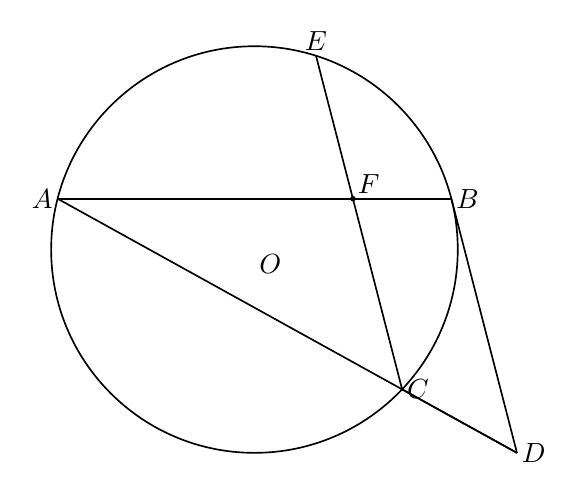
\begin{tikzpicture}[scale=1.25, semithick, every node/.style={inner sep=1.5pt}]
  \coordinate (O) at (0,0);
  \draw (O) circle (2.0656);
  \coordinate (A) at (-2,0.5164);
  \coordinate (B) at (2,0.5164);
  \coordinate (C) at (1.5,-1.4201);
  \coordinate (E) at (0.625,1.9688);
  \coordinate (F) at (1,0.5164);
  \coordinate (D) at (2.6667,-2.0656);
  \draw (A) -- (B);
  \draw (A) -- (D);
  \draw (C) -- (D);
  \draw (B) -- (D);
  \draw (C) -- (E);
  \fill (F) circle (0.8pt);
  \node[left] at (A) {$A$};
  \node[right] at (B) {$B$};
  \node[right] at (C) {$C$};
  \node[right] at (D) {$D$};
  \node[above] at (E) {$E$};
  \node[above right] at (F) {$F$};
  \node[below right] at (O) {$O$};
\end{tikzpicture}
\end{center}
\nopagebreak[4]
\end{question}
\begin{question}
\gkti{14}已知函数 $y=\dfrac{|x^2-1|}{x-1}$ 的图象与函数 $y=kx$ 的图象恰有两个交点，则实数 $k$ 的取值范围是\gkblank{}。

\end{question}
\gkpart{三、解答题}

\begin{question}
\gkti{15}某地区有小学 $21$ 所，中学 $14$ 所，大学 $7$ 所，现采用分层抽样的方法从这些学校中抽取 $6$ 所学校对学生进行视力调查。

（1） 求应从小学、中学、大学中分别抽取的学校数目；

（2） 若从抽取的 $6$ 所学校中随机抽取 $2$ 所学校做进一步数据分析，
① 列出所有可能的抽取结果；
② 求抽取的 $2$ 所学校均为小学的概率。

\end{question}
\begin{question}
\gkti{16}在 $\triangle ABC$ 中，内角 $A$，$B$，$C$ 所对的边分别是 $a$，$b$，$c$。已知 $a=2$，$c=\sqrt2$，$\cos A=-\dfrac{\sqrt2}4$。

（1） 求 $\sin C$ 和 $b$ 的值；

（2） 求 $\cos\left(2A+\dfrac\pi3\right)$ 的值。

\Needspace{0.4\textheight}
\end{question}
\begin{question}
\gkti{17}如图，在四棱锥 $P-ABCD$ 中，底面 $ABCD$ 是矩形，$AD\perp PD$，$BC=1$，$PC=2\sqrt3$，$PD=CD=2$。

（1） 求异面直线 $PA$ 与 $BC$ 所成角的正切值；

（2） 证明：平面 $PDC\perp$ 平面 $ABCD$；

（3） 求直线 $PB$ 与平面 $ABCD$ 所成角的正弦值。
\nopagebreak[4]
\begin{center}% 2012 年天津卷文科第 17 题：四棱锥 P-ABCD，底面 ABCD 为矩形，AD⊥PD。
% 来源 PDF：普通高考/2012/2012天津文.pdf，第 2 页（印面 778）第 1 栏。
% 重绘依据：原图为斜二测式透视：A、B 在前，C、D 在后，P 在上方偏左；
%   实线 PA、PB、PC、PD、AB、BC，虚线 AD、CD、AC。
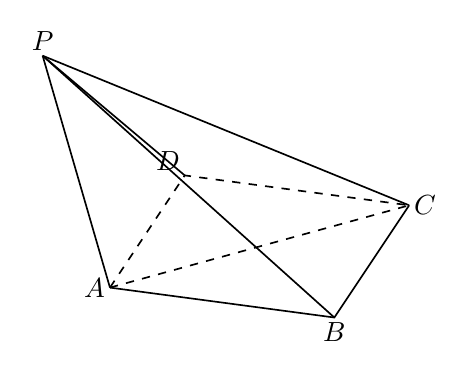
\begin{tikzpicture}[scale=0.95, semithick, every node/.style={inner sep=1.5pt}]
  \coordinate (A) at (0.4,0.5);
  \coordinate (B) at (3.4,0.1);
  \coordinate (C) at (4.4,1.6);
  \coordinate (D) at (1.4,2.0);
  \coordinate (P) at (-0.5,3.6);
  \draw (P) -- (A);
  \draw (P) -- (B);
  \draw (P) -- (C);
  \draw (P) -- (D);
  \draw (A) -- (B) -- (C);
  \draw[dashed] (A) -- (D) -- (C);
  \draw[dashed] (A) -- (C);
  \node[left] at (A) {$A$};
  \node[below] at (B) {$B$};
  \node[right] at (C) {$C$};
  \node[above left] at (D) {$D$};
  \node[above] at (P) {$P$};
\end{tikzpicture}
\end{center}
\nopagebreak[4]
\end{question}
\begin{question}
\gkti{18}已知 $\{a_n\}$ 是等差数列，其前 $n$ 项和为 $S_n$，$\{b_n\}$ 是等比数列，且 $a_1=b_1=2$，$a_4+b_4=27$，$S_4-b_4=10$。

（1） 求数列 $\{a_n\}$ 与 $\{b_n\}$ 的通项公式；

（2） 记 $T_n=a_1b_1+a_2b_2+\cdots+a_nb_n$，$n\in\mathbf N^*$，证明：$T_n-8=a_{n-1}b_{n+1}$（$n\in\mathbf N^*$，$n>2$）。

\end{question}
\begin{question}
\gkti{19}已知椭圆 $\dfrac{x^2}{a^2}+\dfrac{y^2}{b^2}=1$（$a>b>0$），点 $P\left(\dfrac{\sqrt5}5a,\dfrac{\sqrt2}2a\right)$ 在椭圆上。

（1） 求椭圆的离心率；

（2） 设 $A$ 为椭圆的左顶点，$O$ 为坐标原点。若点 $Q$ 在椭圆上且满足 $|AQ|=|AO|$，求直线 $OQ$ 的斜率的值。

\end{question}
\begin{question}
\gkti{20}已知函数 $f(x)=\dfrac13x^3+\dfrac{1-a}2x^2-ax-a$，$x\in\mathbf R$，其中 $a>0$。

（1） 求函数 $f(x)$ 的单调区间；

（2） 若函数 $f(x)$ 在区间 $(-2,0)$ 内恰有两个零点，求 $a$ 的取值范围；

（3） 当 $a=1$ 时，设函数 $f(x)$ 在区间 $[t,t+3]$ 上的最大值为 $M(t)$，最小值为 $m(t)$，记 $g(t)=M(t)-m(t)$，求函数 $g(t)$ 在区间 $[-3,-1]$ 上的最小值。

\clearpage

\end{question}